% ============================================================
%  Figure 10 — Long-window fit quality (L = 500 ms)
%  Biased fit: I_ss_fit=1.285, tau_ac_fit=1.14
% ============================================================
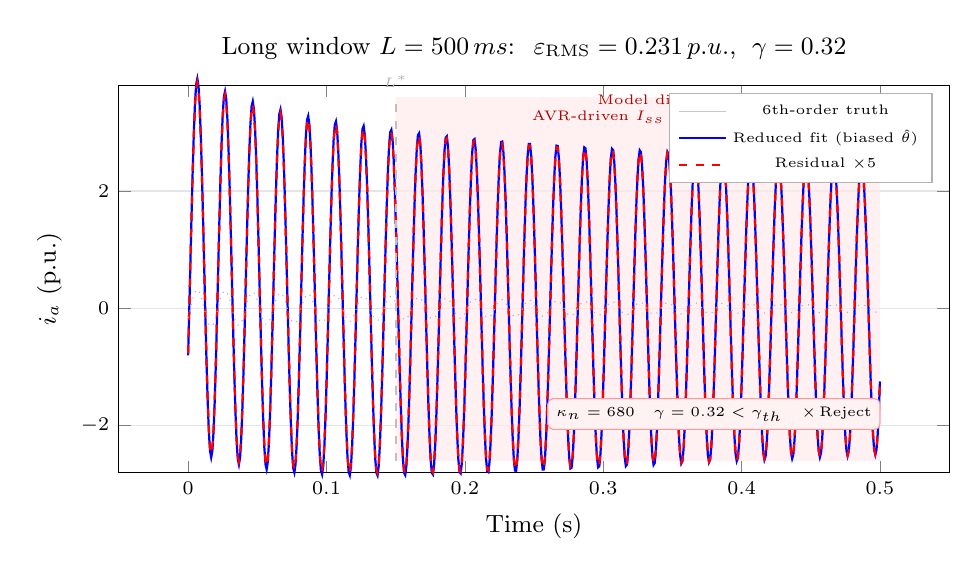
\begin{tikzpicture}
\begin{axis}[
  width=\columnwidth, height=6.5cm,
  domain=0:0.50, samples=600,
  xlabel={Time (s)},
  ylabel={$i_a$ (p.u.)},
  ymin=-2.8, ymax=3.8,
  ymajorgrids=true, grid style={gray!20},
  label style={font=\small},
  tick label style={font=\scriptsize},
  title={Long window $L = 500\,\text{ms}$:\;
         $\varepsilon_{\mathrm{RMS}} = 0.231\,\text{p.u.}$,\;
         $\gamma = 0.32$},
  title style={font=\small},
  legend style={at={(0.98,0.98)}, anchor=north east,
                font=\tiny, fill=white, draw=black!30},
  clip=false
]

% Divergence region shading
\addplot[fill=red!8, draw=none, opacity=0.7]
  coordinates {(0.15,-2.6)(0.50,-2.6)(0.50,3.6)(0.15,3.6)} \closedcycle;

% 6th-order truth
\addplot[blue, thick, solid] {
  (1.35*(1+0.15*(1-exp(-x/0.5))) + 1.85*exp(-x/0.83))
  * sin(deg(314.16*x) - 30)
  + 1.60*0.5*exp(-x/0.07)
};

% Biased reduced fit (I_ss=1.285, tau_ac=1.14 — LM overfit to compensate)
\addplot[red, dashed, thick] {
  (1.285 + 1.85*exp(-x/1.14)) * sin(deg(314.16*x) - 30)
  + 1.60*0.5*exp(-x/0.07)
};

% Residual x5
\addplot[gray!60, dotted] {
  5 * ((1.35*(1+0.15*(1-exp(-x/0.5))) - 1.285
       + (1.85*exp(-x/0.83) - 1.85*exp(-x/1.14)))
       * sin(deg(314.16*x) - 30))
};

\legend{6th-order truth, Reduced fit (biased $\hat{\bm\theta}$),
        Residual $\times 5$};

% Annotation: divergence note
\node[font=\tiny, red!70!black, align=center]
     at (axis cs:0.35, 3.4)
     {Model divergence:\\AVR-driven $I_{ss}$ rise not captured};

% Annotation box: reject
\node[draw=red!40, fill=red!5, rounded corners=2pt,
      font=\tiny, align=left, inner sep=3pt]
  at (axis cs:0.38, -1.8)
  {$\kappa_n = 680$\quad $\gamma = 0.32 < \gamma_{th}$\quad
   $\times$\,Reject};

% Validity boundary
\draw[thick, gray!50, dashed] (axis cs:0.15, -2.6) -- (axis cs:0.15, 3.6);
\node[above, font=\tiny, gray!60] at (axis cs:0.15, 3.6) {$L^*$};

\end{axis}
\end{tikzpicture}
